\subsection{Pantalla: Gestionar Temas Transversales}
\subsubsection{Objetivo}
	El mapa de navegación se muestra en la Figura~\ref{fig:mapaNavegacionCUG2}

   \begin{figure}[hbpt!]
 		\centering
 			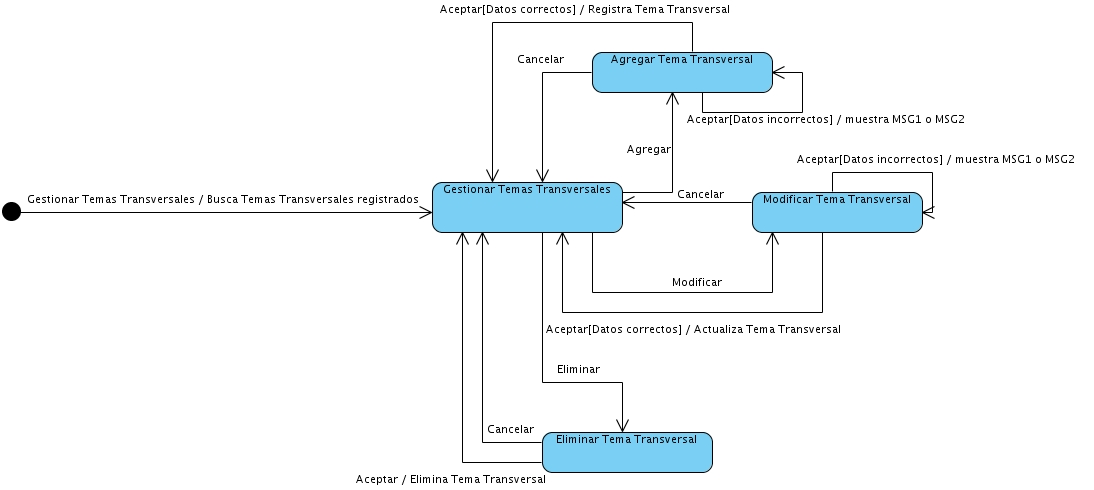
\includegraphics[width=0.8\textwidth]{images/CUG2/MapaNavegacion.jpg}
 		\caption{Mapa de navegacion para el CU G2 Gestion de Temas Transversales.}
		\label{fig:mapaNavegacionCUG2}
 	\end{figure}

\subsubsection{Objetivo}
  Mostrar la información correspondiente a los Tipos de Aviso con el fin de mantener actualizada la información, ver Figura~\ref{IUGestTemasTransversales}. Viene de Menú Gestión de Catálogos.

%\subsubsection{Diseño}%[h]
\IUfig[0.6]{CUG2/gestionarTemasTransversales.png}{IUGestTemasTransversales}{Gestionar Temas Transversales}	

\subsubsection{Salidas}
  En esta pantalla se muestran los Datos de los Temas Transversales registrados en una tabla, ordenados por Nombre en forma ascendente.

\subsubsection{Comandos}
\begin{itemize}
 \item Al presionar \IUbutton{
\includegraphics[scale=0.15]{images/icons/agregar.png}} el sistema muestra la pantalla \IUref{IUAgregarTemaTransversal}{Agregar Tema Transversal} para poder agregar un Tema Transversal.
 \item Al presionar \IUbutton{
\includegraphics[scale=0.1]{images/icons/editar.png}} el sistema muestra la pantalla \IUref{IUModificarTemaTransversal}{Modificar Tema Transversal} para poder modificar un Tema Transversal.
 \item Al presionar \IUbutton{
\includegraphics[scale=0.1]{images/icons/eliminar.png}} el sistema muestra la pantalla \IUref{IUEliminarTemaTransversal}{Eliminar Tema Transversal} para poder eliminar un Tema Transversal.

\end{itemize}

\subsubsection{Mensajes}
  Ninguno.

